% =============================================================
%  800 VDC Architecture for AI Infrastructure — Report
%  Based on NVIDIA's 800 VDC Architecture for Next-Generation AI Infrastructure
%  Uses the shared American Terawatt report style.
%  Compile:  pdflatex datacenter.tex   (run twice for ToC / references)
% =============================================================
\documentclass[11pt,a4paper]{article}

% Shared style lives in the repo-level template folder
\usepackage[corporate]{../../template/attemplate}
\usepackage{listings}
\usepackage{booktabs}
\usepackage{rotating}
\usepackage{longtable}

% TikZ libraries used by architecture diagrams
\usetikzlibrary{arrows.meta,positioning,calc,shapes.geometric,fit}

% ---- Shell / code listing style ----------------------------------------------
\lstdefinestyle{atshell}{
  basicstyle=\ttfamily\fontsize{8.5}{11}\selectfont\color{atFg},
  backgroundcolor=\color{atBgSubtle},
  frame=single,
  rulecolor=\color{atBorder},
  framesep=5pt,
  breaklines=true,
  breakindent=0pt,
  postbreak=\mbox{\textcolor{atBorderStrong}{$\hookrightarrow$}\space},
  columns=flexible,
  keepspaces=true,
  showstringspaces=false,
  commentstyle=\color{atFgMuted}\itshape,
  morecomment=[l]{\#},
  xleftmargin=0pt,
  aboveskip=8pt,
  belowskip=8pt,
}
\lstset{style=atshell}

\newcommand{\cmd}[1]{\texttt{\small #1}}

% ---- Report metadata ---------------------------------------------------------
\reporttitle{800 VDC Architecture for AI Infrastructure}
\reportsubtitle{The Architectural Imperative of 800 VDC and Integrated Energy Storage}
\atEyebrow{Datacenter Power Systems}
\atAbstract{Analysis of 800 VDC power distribution architectures for next-generation AI datacenter infrastructure, covering the exponential power demands driven by GPU workloads, energy storage strategies for load swing mitigation, grid interconnection requirements, and facility-level reference designs.}
\reportauthor{Based on work by Jared Huntington \& Mike Tu (NVIDIA)}
\reportdocnumber{ATW-REP-DC-001}
\reportrevision{0.1}
\reportstatus{Draft}
\reportdate{\today}
\reportconfidentiality{Confidential}

\begin{document}

\makecover

\revisionhistory{
  \revrow{0.1}{\today}{Eugen Starschich}{Initial document derived from NVIDIA whitepaper}
}

\newpage
\tableofcontents
\clearpage

% ---- Body --------------------------------------------------------------
\section{Introduction}

Only a few years ago, data centers were built around the compute space, vast data halls of servers, with power and cooling systems taking up a smaller share of the footprint. Then came the GPU revolution, transforming the data center into ``AI Factories''. As shown in Figure~\ref{fig:power-generation}, GPU racks are approaching 100 times greater power density compared to web servers and are increasing in power at a near-exponential pace, flipping the balance. Power infrastructure, once secondary, now rivals or even exceeds the space dedicated to compute.

\begin{figure}[h]
\centering
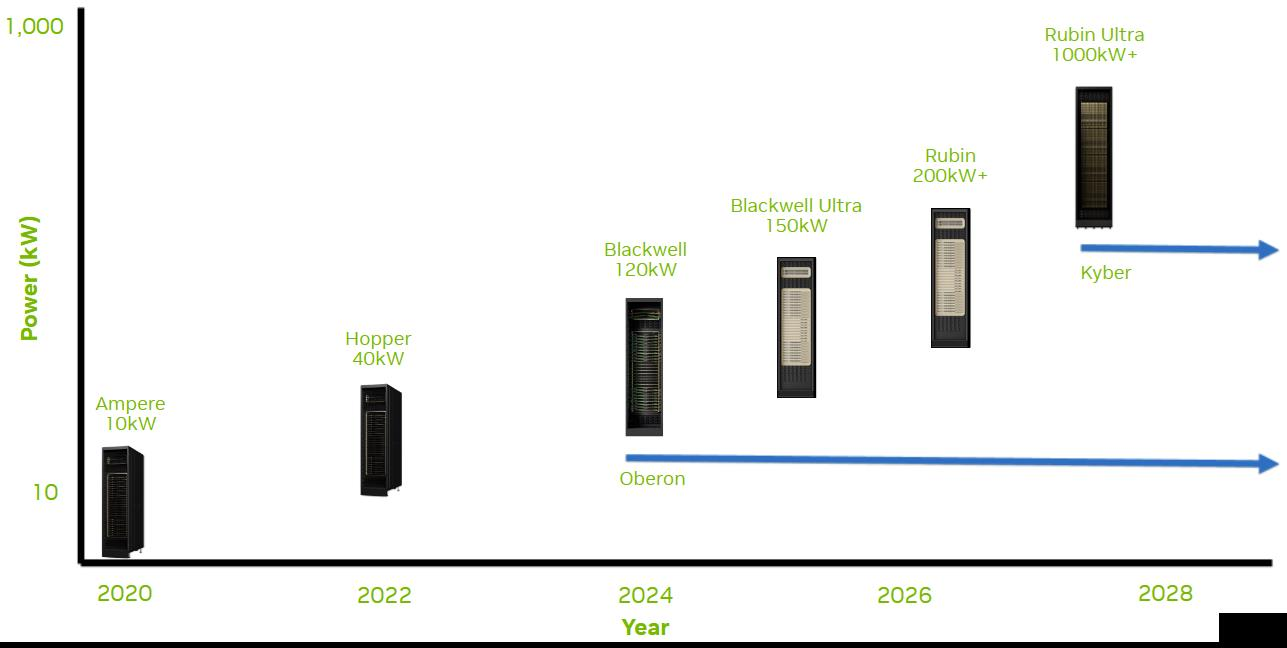
\includegraphics[width=0.8\textwidth]{figures/figure_p3_i1.jpeg}
\caption{Increasing Power Generation over Generation}
\label{fig:power-generation}
\end{figure}

As CPUs or GPUs are improved, there is typically an incremental increase in the GPU thermal design point (TDP) for power of 20\% generation over generation. This leads to an increase in power required per server over time. Nvidia's NVLink allows multiple GPUs to be networked together to effectively act as one large synchronous GPU and provide a significant improvement in performance when compared to operating over Ethernet connections. This networking of GPUs is most effective when connected over copper from both a power and cost standpoint, but at the expense of a limited reach due to signal integrity. Since the highest performance can be achieved when more GPUs are on the same copper domain with a limited reach, the maximum performance is tied to maximum power density. This means power increases are no longer 20\% generation over generation, but can easily be 2x, 4x or 8x with the increase in NVLink networking domain size.

\begin{figure}[h]
\centering
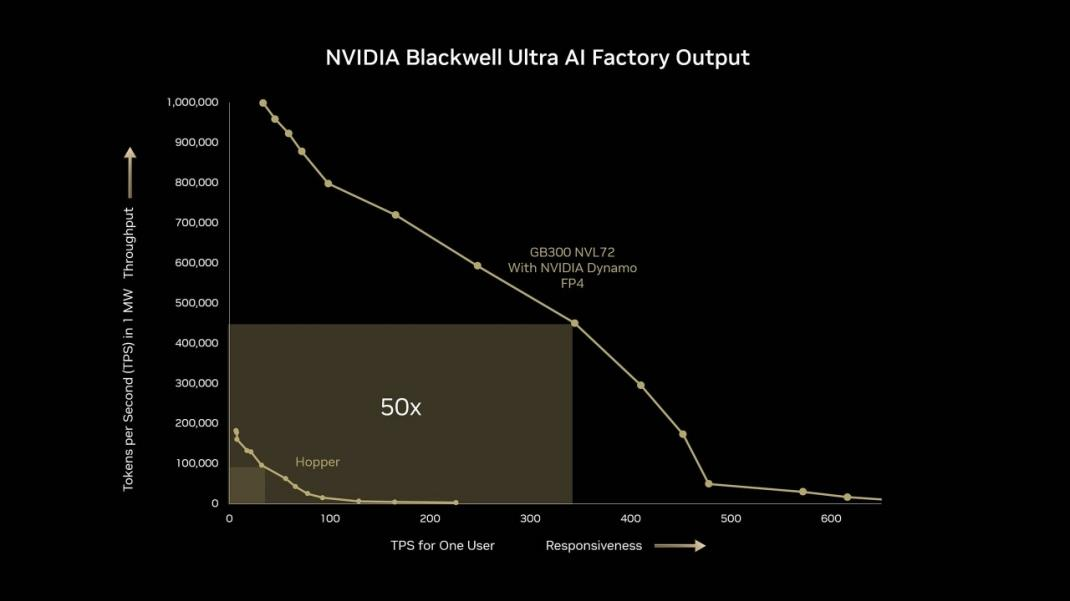
\includegraphics[width=0.8\textwidth]{figures/figure_p4_i1.jpeg}
\caption{A 75\% increase in TDP power, but a 50x increase in performance}
\label{fig:performance-increase}
\end{figure}

An example in Figure~\ref{fig:performance-increase} above is the performance increase from Hopper to GB300. The TDP power increased by 75\%, but the performance increased 50x with these changes. This also led to a 3.4x increase in rack power density going from an 4x8 GPU NVLink domains (32 in the rack) to a 72 GPU NVLink domain. As GPU packing and packaging improves and networking topologies move to larger domain sizes, this power density can continue to increase.

This increase in power generation over generation and with NVLink domain drives a much more rapid increase in power than has been seen in the past with GPUs. A secondary goal is to remove as many power components from the NVLink domain radius as possible since this is the highest value real estate in the rack for performance. This combination of driving to higher power level and pushing the power components away from the GPUs drives requirements for a different rack power architecture.

To meet these unprecedented demands, 800 VDC has emerged as the optimal architecture for next-generation power distribution. It allows for minimizing the conversion and routing volume in the compute space while minimizing datacenter distribution losses and total end to end conversion stages. 800 VDC significantly reduces current, copper use, and cable bulk compared to 54 VDC inside the rack or facility level 480 VAC systems, while remaining safe and scalable. It benefits from the growing maturity of Silicon Carbide (SiC) and Gallium Nitride (GaN) power conversion devices and the widespread adoption of 800 VDC systems in the electric vehicle (EV) industry. This enables seamless, end-to-end integration from grid to rack, higher power density beyond 1 MW.

Datacenters historically consisted of thousands of servers running diverse workloads. With GPUs these workloads can be synchronous across the datacenters leading to massive load swings in very short time intervals. Energy storage can be used to mitigate these swings. This rapid shift in datacenter power infrastructure requirements puts the industry at a crossroads. To keep up with future GPU demands, we need to rethink how we deliver power. This leads us to the next-generation distribution system that is more efficient, scalable, and ready for the extremely dynamic AI workloads. Integrating 800 VDC architectures with energy storage is key to future-proofing AI Factories for the era ahead.

\section{Load Swings and Energy Storage}

One consequence of GPUs being synchronized is that their workloads and therefore power profiles are also synchronized. This has been a problem in supercomputers for decades but is now becoming widely understood as a challenge during AI factory deployments. During a typical LLM workload there are intervals of intense matrix computation followed by intervals exchanging data. Unmitigated, this leads to rapid swings from idle at approximately 30\% of rack power to 100\% power utilization. This becomes a problem not only for the rack power distribution, but with large enough cluster sizes, it is an issue at the datacenter level and even the power grid.

\begin{figure}[h]
\centering
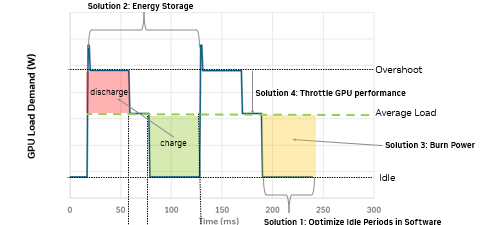
\includegraphics[width=0.8\textwidth]{figures/figure_p5_i1.png}
\caption{Energy storage to flatten the load demand}
\label{fig:load-flatten}
\end{figure}

To deal with these load swings there are multiple approaches that can be taken as seen in Figure~\ref{fig:load-flatten}: Energy storage to flatten the load demand.

\begin{description}
\item[Solution 1 -- Optimize Idle Periods in Software] If these idle periods can be minimized in software this is the ideal solution since it reduces datacenter power requirements.

\item[Solution 2 -- Energy storage] This is an energy efficient method to deal with these load swings is to use energy storage. Energy storage allows charging during the idle periods and discharging during the peaks to low pass filter the rack current demand. This energy storage can come in multiple forms, electrolytic capacitors, supercapacitors, batteries, etc.

\item[Solution 3 -- Burn Power] This is done in the Nvidia GPU via the Power Smoothing feature. This allows for burning power after a delay so that power only burned after the limit of the energy storage has been reached. This is not ideal on it's own, but in conjunction with energy storage can provide a backstop for longer idle periods than the local energy storage can maintain.

\item[Solution 4 -- Throttle GPU performance to reduce peaks] These software controls are available in the Nvidia GPUs, but this is not ideal because it can reduce performance with some workloads.
\end{description}

All 4 solutions can be used together to provide a comprehensive load swing mitigation strategy. Ideally the energy storage is used to cover a majority of the load swing durations while burning power and throttling performance only act as a backstop in corner cases.

\begin{figure}[h]
\centering
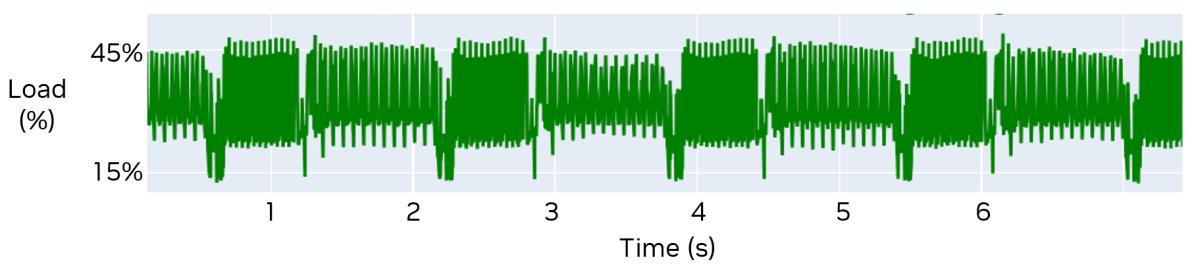
\includegraphics[width=0.8\textwidth]{figures/figure_p6_i1.jpeg}
\caption{GPU Load Swings during an LLM workload}
\label{fig:gpu-load-swing}
\end{figure}

Looking across the GPU workload in Figure~\ref{fig:gpu-load-swing} are events at multiple timescales. Looking at the overall system, there are grid level fluctuation requirements and the GPU load demand requirements. Energy storage needs to fill the gap between these two conflicting requirements; the grid needs a stable predictable load, and the GPU needs a very dynamic source.

GPU overshoots known as the Electrical Design Point (EDPp) and peak power consumption and typical workload idle periods are in the range of up to 100ms, checkpointing can take 1 to 5 seconds, and then the workload ramp up and ramp down needs to occur over several minutes. In addition, depending on the use case, energy storage might be required as transition power to ensure that the load remains operational even during the transfer to a backup power source after a loss of primary power.

\begin{figure}[h]
\centering
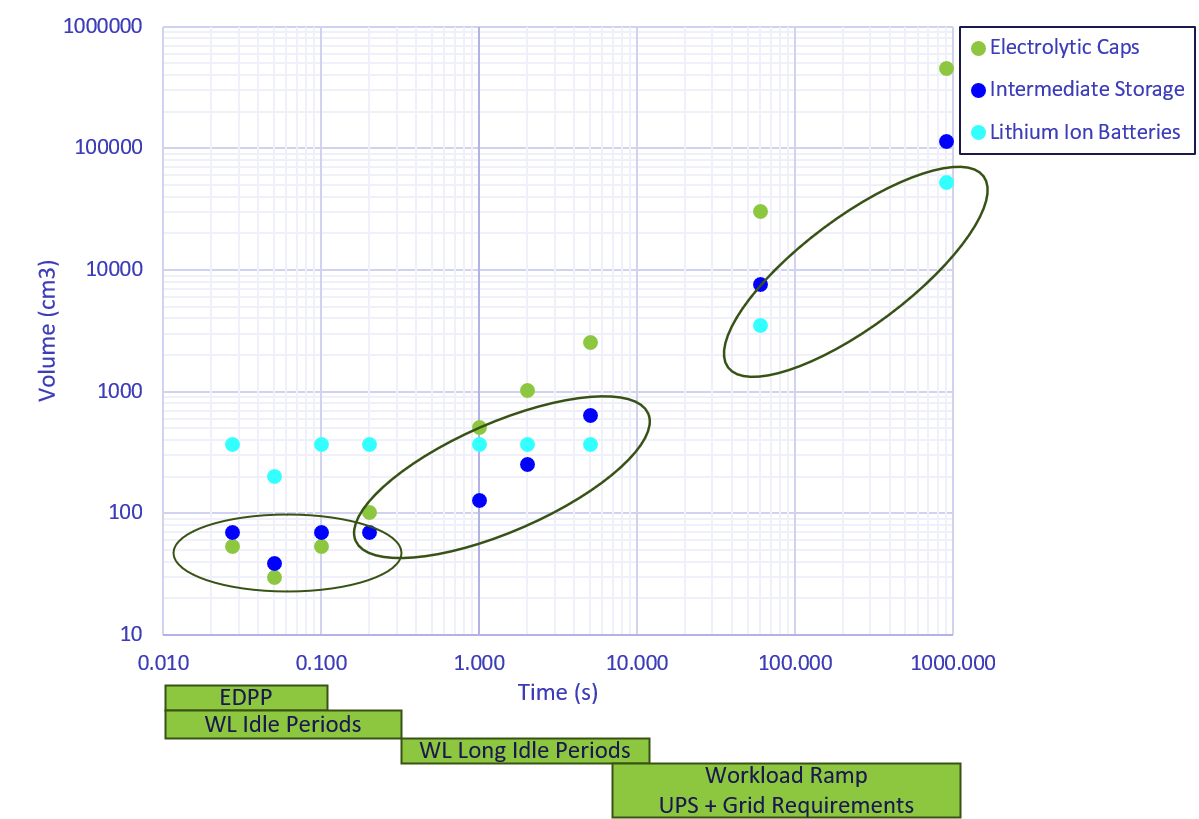
\includegraphics[width=0.8\textwidth]{figures/figure_p7_i1.png}
\caption{Volume of energy storage by technology vs. time duration}
\label{fig:storage-volume}
\end{figure}

Figure~\ref{fig:storage-volume} above shows volume of different energy storage solutions vs. time. Volumetrically electrolytic capacitors are a good solution for anything below 100 ms. There is a mix of solutions that are more optimized for the period between 100 ms and 10 seconds and then beyond this timescale batteries are the better volumetric solution. Mitigating the load swings as close as possible to the GPU is desired to keep slew rates on the datacenter manageable as well as to reduce the RMS current increases. A square wave with a 50\% duty cycle and a 50\% peak over the average then going back to idle will result in a 25\% increase in RMS losses. Equipment in the datacenter needs to be sized to handle the peak current of the rack as well as the increase in RMS losses so reducing these peaks as close as possible to the GPU is valuable for reducing overall datacenter equipment costs and impacts.

\section{Grid Interconnect Requirements}

The load demands described above provide unprecedented interconnection challenges due to the scale and volatility of their power demand. Grid operators are starting to require greater load flexibility, controllability, and predictability to maintain power grid stability, avoid overbuilding for peak demand, and reduce stress on transmission infrastructure.

Unmitigated step changes in AI workloads, especially from large, synchronized GPU clusters, can cause rapid voltage and frequency deviations outside of acceptable bands. These events risk violating interconnection requirements, degrading grid performance, and triggering delays or denials in interconnection approvals.

To secure timely grid access and ensure stable long-term operation, AI compute loads should incorporate compute settings adjustments, active power conditioning, and grid-compliance controls over Ethernet, including:

\begin{itemize}
\item \textbf{Energy storage systems:} energy storage (longer and shorter duration) with fast, real-time power compensation to stabilize power consumption, control ramp rates, and mitigate large step changes.

\item \textbf{GPU performance tuning and workload pacing:} Adjust compute firmware and operational settings to smooth rapid power fluctuations, limit cycle-to-cycle ramp rates, and suppress peak power behavior.

\item \textbf{Coordinated control strategies:} Integrate storage, compute, and facility power distribution systems to ensure compliance with utility requirements for ramp rate, transient stability, harmonics/flicker, and voltage ride-through (VRT), while supporting overall grid stability.
\end{itemize}

Looking ahead, AI Factories have the potential to evolve into grid-supporting assets rather than operating solely as large, passive loads. By adopting advanced capabilities, industry partners can help ensure that AI infrastructure not only scales sustainably but also strengthens the energy systems it depends on.

\begin{itemize}
\item \textbf{Grid-forming and fast-response controls via Ethernet} that actively support voltage and frequency stability during grid disturbances.

\item \textbf{Enhanced fault ride-through capability for internal IT loads,} surpassing current ITIC curve expectations by referencing ERCOT Voltage Ride-Through (VRT) requirements for large electronic loads, to maintain critical operations and support grid recovery during voltage sags or faults.

\item \textbf{Real-time power support,} delivering supplemental power when the grid is under stress and absorbing excess power when available, helping smooth sudden changes and maintain utility grid stability.

\item \textbf{Resilient system designs and operational practices} that position AI Factories as contributors to overall grid reliability and resilience, enabling faster, more predictable scaling of deployments.
\end{itemize}

To ensure grid stability and power quality in high-density AI Factories, energy storage must be strategically deployed at both ends of the electrical architecture. Energy storage, such as a Battery Energy Storage System (BESS), is placed adjacent to the utility interconnection and on-prem generation to manage steady-state power fluctuations from large-scale GPU clusters. The BESS provides load averaging, grid-forming support, and transitional power during utility-to-generator switching events. At the other end, short-duration storage such as capacitors are integrated near the compute racks to mitigate fast dynamic power behavior (as fast as 400 microseconds) generated by AI workloads. These devices serve to limit ramp rates and absorb power peaks and troughs, ensuring a stable and predictable 800 VDC supply to sensitive compute infrastructure. This dual-layered storage strategy is critical to meeting the performance and reliability demands of AI-native power systems.

Interconnection approvals remain a major bottleneck for AI Factory deployment, largely due to the unpredictable nature of GPU-driven load swings. Industry collaboration is needed to establish standardized load behavior profiles, response metrics, and conditioning requirements. Clear alignment on ramp-rate limits, load flexibility, and energy storage integration will help utilities evaluate AI Factory projects more confidently, speeding approvals and enabling faster, more scalable deployment.

Energy storage must be treated as a core element of AI Factory architecture. Beyond stabilizing GPU loads, its standardized roles should cover transient mitigation, backup source, and load shaping, with common integration interfaces for seamless deployment at rack, row, or facility level. This approach ensures interoperability with power conversion systems and grid interconnection schemes, improves equipment utilization, and enables reliable scaling without compromising compute performance.

\section{Power Distribution Options}

Traditional 415V or 480V 3-phase AC power systems have long supported data center growth. However, as compute rack power density approaches and exceeds the megawatt scale, these systems are reaching their practical limits.

\begin{itemize}
\item \textbf{Whip Size and Ampacity:} Typical AC whips are rated at 60 A or 100 A, constrained by thermal limits and connector standards such as IEC 60309.

\item \textbf{Rack Power Inlets:} Higher rack power demands require more and/or larger input connections, consuming valuable rack space and complicating cable management.

\item \textbf{Power Asset Coordination:} Managing and protecting multiple AC feeds adds design complexity and increases the equipment footprint.
\end{itemize}

As rack-level power rises, the use of traditional AC distribution results in greater system complexity, more components, and reduced scalability, driving up both capital and operational costs for next-generation deployments.

Looking at the amount of power that can be transferred through a fixed wire gauge rated at 48A continuous vs. voltage, the table below shows that going from 415 VAC to 800 VDC allows for 157\% more power to be transmitted through the same cross-sectional area of copper. A common method to get more power out of the same infrastructure in North America is to use 480 VAC, but that only gives a 16\% improvement in infrastructure. Looking further out to 1500 VDC distribution gives a 382\% increase in power through the same conductor sizes.

\begin{table}[h]
\centering
\caption{AC vs. DC Power Cable Comparison}
\label{tab:ac-dc-comparison}
\begin{tabular}{llcc}
\toprule
\textbf{Voltage} & \textbf{Wires} & \textbf{\begin{tabular}[c]{@{}c@{}}Power per cable\\ diameter (kW/mm\textsuperscript{2})\end{tabular}} & \textbf{\begin{tabular}[c]{@{}c@{}}Power Increase\\ ref. 415 VAC\end{tabular}} \\
\midrule
415 VAC   & 4 (P1,P2,P3,PE) & 0.6 & + 0\%  \\
480 VAC   & 4 (P1,P2,P3,PE) & 0.8 & + 16\% \\
800 VDC   & 3 (POS,RTN,PE)  & 1.7 & + 157\%\\
1500 VDC  & 3 (POS,RTN,PE)  & 3.1 & + 382\%\\
\bottomrule
\end{tabular}
\end{table}

\subsection*{Transitioning to 800 VDC Distribution}

Moving to 800 VDC facility-level distribution addresses these challenges and offers several key advantages:

\begin{itemize}
\item \textbf{Simplified Power Interface to IT:} As GPU rack power density rapidly outpaces traditional web servers, reaching megawatt levels, the existing 415/480 VAC cables and connection schemes are no longer viable. A shift to 800 VDC enables a streamlined physical interface to the rack, dramatically reducing the number of cables and components needed. This simplifies installation, minimizes space use, and improves operational agility: critical factors as power infrastructure now rivals compute in footprint and complexity.

\item \textbf{Streamlined System Architecture:} Migrating AC/DC conversion upstream from the IT rack to the facility level, and ultimately to direct Medium Voltage AC-to-DC conversion, eliminates unnecessary stages. This results in a leaner, more efficient architecture that reduces equipment layers, cost, and space, while increasing reliability and deployment speed as key enablers for future-ready AI Factories.

\item \textbf{Direct Compatibility with GPU Racks:} While facility-level DC distribution can be designed to support a range of voltage architectures, the final delivery to compute must maintain an 800 VDC differential. This ensures seamless interoperability between facility power infrastructure and rack-level hardware, simplifying integration, reducing customization needs, and enabling a unified deployment strategy across AI Factory deployments.
\end{itemize}

\subsection*{Adjacent Industry Blueprints for LVDC Distribution}

Several adjacent industries have already proven the viability of LVDC power distribution, offering valuable reference points for AI Factory power systems:

\begin{itemize}
\item \textbf{Electric Vehicles (EV):} EV platforms have evolved from 400 VDC to 800 VDC and higher, as seen in Porsche, Hyundai, and GM vehicles. Their systems emphasize fast charging, high power density, reduced copper usage, and feature high-efficiency rectifiers, large-ampacity portable cables, advanced safety connectors, and fault-tolerant protection schemes.

\item \textbf{Photovoltaics (PV):} Utility-scale PV farms typically operate at 1000-1500 VDC, supported by a mature ecosystem of DC-rated switchgear, fuses, and combiner boxes, mostly optimized for outdoor, lower-current applications.

\item \textbf{Rail \& Industrial:} Long-distance LVDC distribution is widely used in transport and industrial microgrids. Examples like Mercedes-Benz Factory 56 leverage DC to integrate renewables and storage, demonstrating scalable and efficient deployment.
\end{itemize}

These industries demonstrate that proven equipment, safety strategies, and operational practices can be adapted for AI Factory use. However, even with this existing maturity, data center deployments require significant engineering adaptation to address much higher power densities and stricter electrical safety requirements unique to hyperscale computing environments.

\subsection*{Facility-Level DC Distribution Options Under Evaluation}

Leading data center operators and cloud service providers are currently assessing several facility-level DC architectures:

\begin{description}
\item[800 VDC (NVIDIA MGX)] Directly supports the Nvidia 800 VDC rack architecture. Benefits from the growing maturity of Gallium Nitride (GaN) and SiC devices-based conversion devices and widespread EV adoption. Enables seamless end-to-end integration for AI compute.

\item[750 VDC (ODCA / VDE-SPEC 90037)] A widely adopted European industrial standard promoting a simplified 2-wire system. Offers short-term compatibility with existing 1000 V-class equipment and electronics. It is gaining traction across transportation and industrial facilities.

\item[$\pm$400 VDC (OCP Standard)] Technically feasible and develops based on the previous 400V DC architecture. However, the midpoint reference creates a 4-wire system, introducing complexity in grounding, phase balancing, and fault detection especially when scaled to datacenter level distribution.

\item[1500 VDC (Potential Future Target)] 1500 VDC is an established limit of the low voltage class under NEC Article 690 (photovoltaic systems) and IEC 62477-1 (industrial converter environments). It is widely used in solar and rail applications for its efficiency in power delivery and ability to reduce copper usage by supporting high power density loads.
\end{description}

However, applying 1500 VDC inside data centers, especially within compute racks, faces significant challenges. Current UL and NEC standards for IT and indoor environments are still evolving, and few certified components exist at this voltage level. In addition, device clearance and creepage distance requirements, component voltage ratings, and arc-flash safety concerns make 1500 VDC difficult to implement safely within confined rack spaces.

As a result, 1500 VDC remains a potential long-term target for large-scale AI factories, while 800 VDC serves as the practical near-term solution, balancing efficiency, conversion stages, equipment availability, and regulatory compliance.

A phased adoption strategy is recommended:
\begin{itemize}
\item \textbf{Near-term:} Deploy 800 VDC to the rack using commercially available 1000 V-class components.
\item \textbf{Potential Long-term:} Transition to 1500 VDC as the in-rack protection device and DC/DC density increases, safety standards solidify, and supporting equipment becomes widely available.
\end{itemize}

\section{800 VDC MGX Architecture}

The above requirements for exponentially increasing power, pushing power out of the NVLink domain, and energy storage for mitigating load swings all come together to define the requirements for the 800 VDC power architecture.

\begin{figure}[h]
\centering
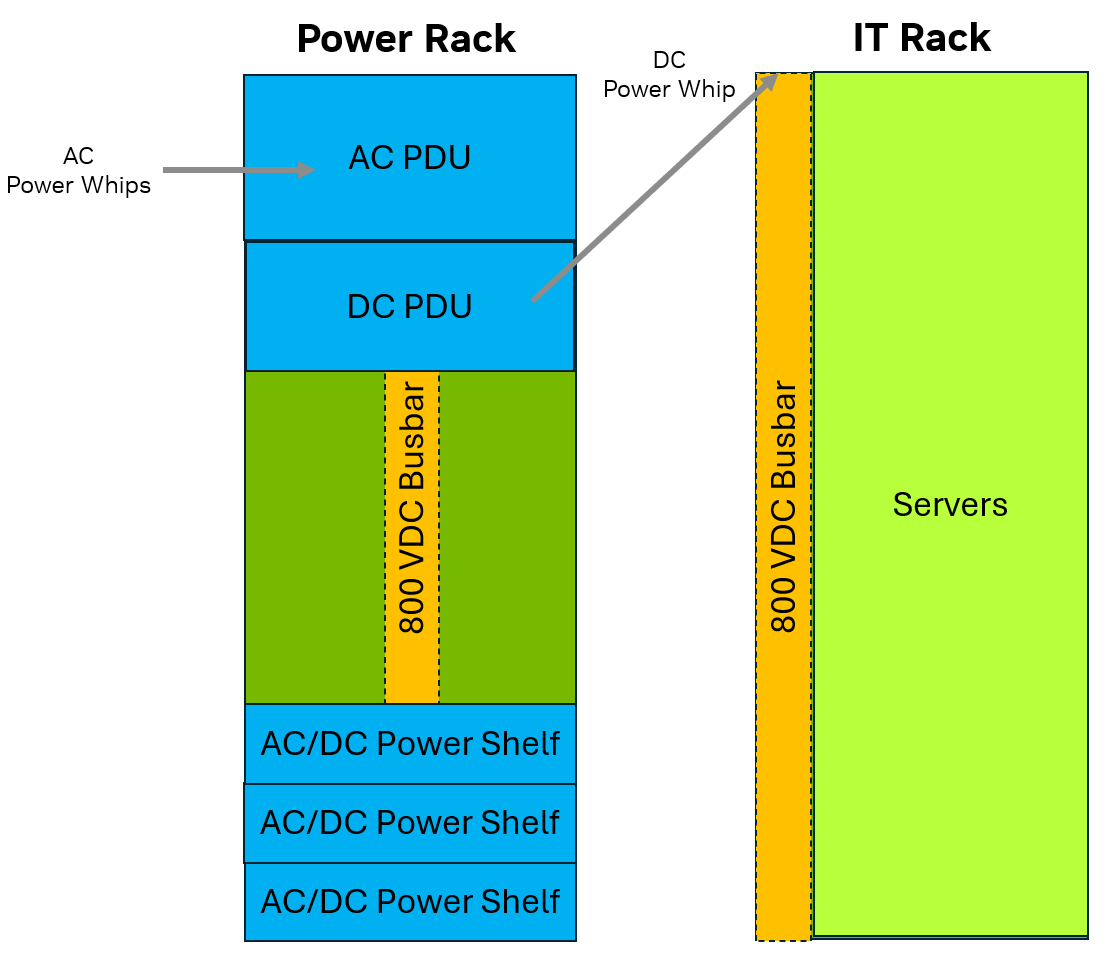
\includegraphics[width=0.8\textwidth]{figures/figure_p12_i1.png}
\caption{800 V MGX Rack Overview}
\label{fig:mgx-rack}
\end{figure}

The overall rack architecture takes 800 VDC directly into the rack and distributes 800 VDC direct to the compute node.

Safety is a critical design feature for the 800V system. Because of this touch-safe connectors are used in all locations that are user accessible. To ensure safety while connecting and disconnecting loads mechanical interlocks are also used in all connectors to ensure that there is no disconnect occurring under load. This helps to minimize the risk of arcing as well as act as a secondary protection ensuring that there are no live accessible parts. These techniques are commonly used in EV chargers which are widely available and used by untrained consumers. The presently planned connectors are leveraging this existing technology and optimizing for a datacenter environment.

To minimize connector sizes and volume of copper, the DC/DC conversion is pushed as close as possible to the GPU. This takes advantage of the 800 VDC to minimize power overhead in the system. The conversion is then done from 800 VDC to 12 VDC and routed a short distance to the voltage regulators.

The 800 VDC is converted directly to 12V with a 64:1 LLC converter and a matrix transformer. This helps to eliminate the separate 400V \textrightarrow{} 50V and 50V \textrightarrow{} 12V converters that are used in the present standard datacenter DC/DC converter power tree giving an additional 1\% in efficiency improvement and a 26\% reduction in area when compared to a multistage approach. This is in the critical area near the GPU.

\begin{figure}[h]
\centering
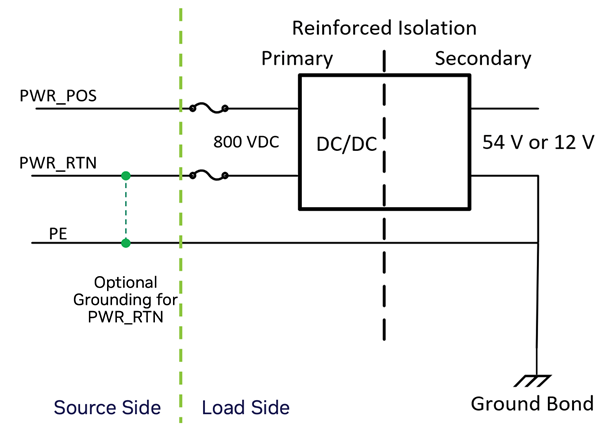
\includegraphics[width=0.8\textwidth]{figures/figure_p13_i1.png}
\caption{DC/DC with symmetrical fusing and hotswap controllers to allow for $\pm$400 VDC or 800 VDC sources}
\label{fig:dc-dc-fusing}
\end{figure}

The IT rack as shown in Figure~\ref{fig:dc-dc-fusing} is also designed to support sources with an 800 VDC total potential with multiple grounding schemes. This makes it so $\pm$400V equipment can be reused to power the rack. This is supported by having fuses on both the high side and low side input of the DC/DC converter and ensuring that both inputs have reinforced isolation from the secondary. To generate the 800 VDC powering the IT rack, there are multiple methods that can be used: side power racks, facility level rectification, medium-voltage rectifier and solid-state transformers.

The decision to implement an 800V DC single-ended configuration was driven by practical considerations around protection device availability and system simplicity when moving to datacenter level distribution. While bipolar configurations such as $\pm$400V DC offer theoretical benefits in grounding and fault isolation, they require specialized three-pole breakers and protection devices that are not widely available in the industry. Developing such components would introduce delays and increase engineering overhead. In contrast, the single-ended 800V DC approach aligns with existing two-pole breaker designs, allowing for faster deployment and reduced complexity. In addition, single ended distribution on the datacenter level does not have any load balancing issues across the positive and return sources.

\begin{figure}[h]
\centering
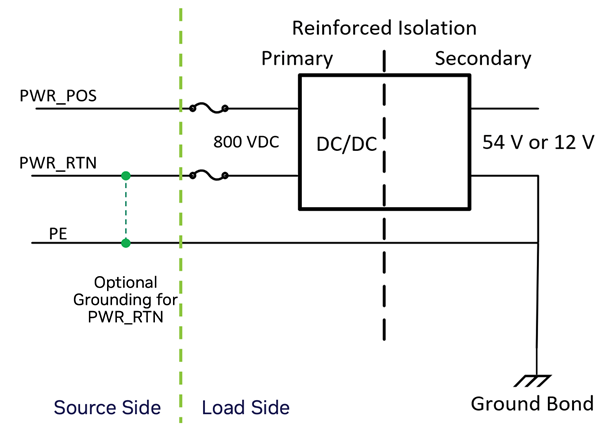
\includegraphics[width=0.8\textwidth]{figures/figure_p13_i1.png}
\caption{Datacenter architecture over time}
\label{fig:evolution}
\end{figure}

Figure~\ref{fig:evolution} illustrates the evolution of data center power distribution from the current 415 VAC architecture to future-ready 800 VDC systems designed to meet AI Factory demands. The existing 415 VAC architecture, shown in the top architecture, involves multiple components: MV step-down transformers, LV switchboards, AC UPS, PDUs, and AC distribution panels (RPP or busway). Power is delivered to each compute rack at 415 VAC, where an in-rack Power Shelf Unit (PSU) converts it to 54 VDC for compute trays and IT equipment. Optional external energy storage may be added to buffer dynamic power swings from the GPU workloads.

To support rising power densities and to provide an adapter to existing facilities, a transitional 800 VDC architecture relocates AC/DC conversion outside the rack. Targeting for White Space retrofit alone with minimal impact, an 800 VDC side power rack is a dedicated power rack containing rectifiers and power distribution units to convert from AC to DC local to each rack. This is required in the near term as components become more readily available to deploy 800 VDC datacenters. This is not the optimal solution end-to-end due to the extra stages of conversion, but it allows moving to higher compute rack densities by pushing power conversion out of the compute rack.

As 800 VDC power distribution equipment and data center operations become more readily available, the side power rack can be replaced by higher power density rectifier and being placed at the upstream of power distribution.

Facility-level AC/DC power rectifiers, as another variation, deliver 800 VDC from low-voltage AC (< 600 V). A typical rectifier string targets \textasciitilde{}1.5 MVA capacity and can be paralleled via a common DC bus. Positioned downstream of LV switchboards or directly under MV/LV transformers, these systems reduce rack-level complexity and support integration of energy storage at the DC output. While step-down transformers remain necessary, rectifiers offer mature, high-efficiency (\textasciitilde{}99\%) solutions widely used in BESS and renewables. This architecture simplifies power delivery and scales to support high-density compute with minimal white space burden.

To meet the rising power demands of AI Factories, NVIDIA is exploring MV Rectifier application (converting MV AC power to 800 VDC) and pursuing Solid State Transformer (SST) technology as future proof facility power distribution solutions. Shown in the bottom architecture, MV Rectifiers and SSTs are targeted to enable direct conversion from Medium Voltage (e.g., 35 kV AC) to 800 VDC, eliminating the need for traditional low-voltage (480 VAC) layers and simplifying the facility power architecture. Size of MV Rectifier and SST can be as large as 7.5 MVA per unit with 98.5\% or better efficiency.

A medium-voltage rectifier is a proven, high-capacity power conversion system widely used in industries like mining, electrolysis, rail, and grid-scale storage for delivering stable, high-power DC. Comprising a step-down transformer, rectification modules, filters, and protection systems, its mature design offers high reliability and supply chain readiness. Compared to the evolving SST, MV rectifiers provide a faster and proven path for quick 800 VDC deployment, making them a strong candidate for near-term AI Factory applications.

The SST system combines a medium-voltage AC intake, power rectification modules, and a DC output distribution section. Its compact and high-power capacity design supports compute rack density growth being scalable and great space saving with DC power equipment. However, scaling SSTs to multi-megawatt capacity presents challenges in the development and reliability of high-power rectification modules and managing thermal and electrical stresses at high density. NVIDIA is actively collaborating with leading industry partners to co-develop SST-based solutions.

The design of the facility-level DC power system must prioritize both resilience and scalability to meet the evolving needs of AI Factories. Resilience requires robust protection schemes, fault isolation strategies, and redundancy across power paths to ensure continuous operation during faults or maintenance. Scalability demands a modular and flexible architecture that enables seamless power expansion without major rework, while upholding safety and efficiency. Key development areas include high-capacity, reliable power rectification, advanced DC distribution boards, coordinated protection with DC devices, clearly defined isolation points for safe maintenance, simplified power interfaces to IT racks, and integrated DC energy storage to mitigate dynamic power swings. Together, these elements form the foundation for long-term reliability and operational agility in high-density compute environments.

\section{Datacenter Reference Design}

NVIDIA's strategy to accelerate ecosystem readiness is by sharing facility-level reference designs that showcase the feasibility of advanced power architectures. These designs are not rigid specifications, but rather illustrative examples to guide ecosystem partners in aligning on scalable, interoperable solutions for AI Factories. They help identify development opportunities and enable faster co-development of supporting technologies. The reference design will evolve in parallel with NVIDIA's compute product specifications to ensure continued alignment and applicability.

\begin{figure}[h]
\centering
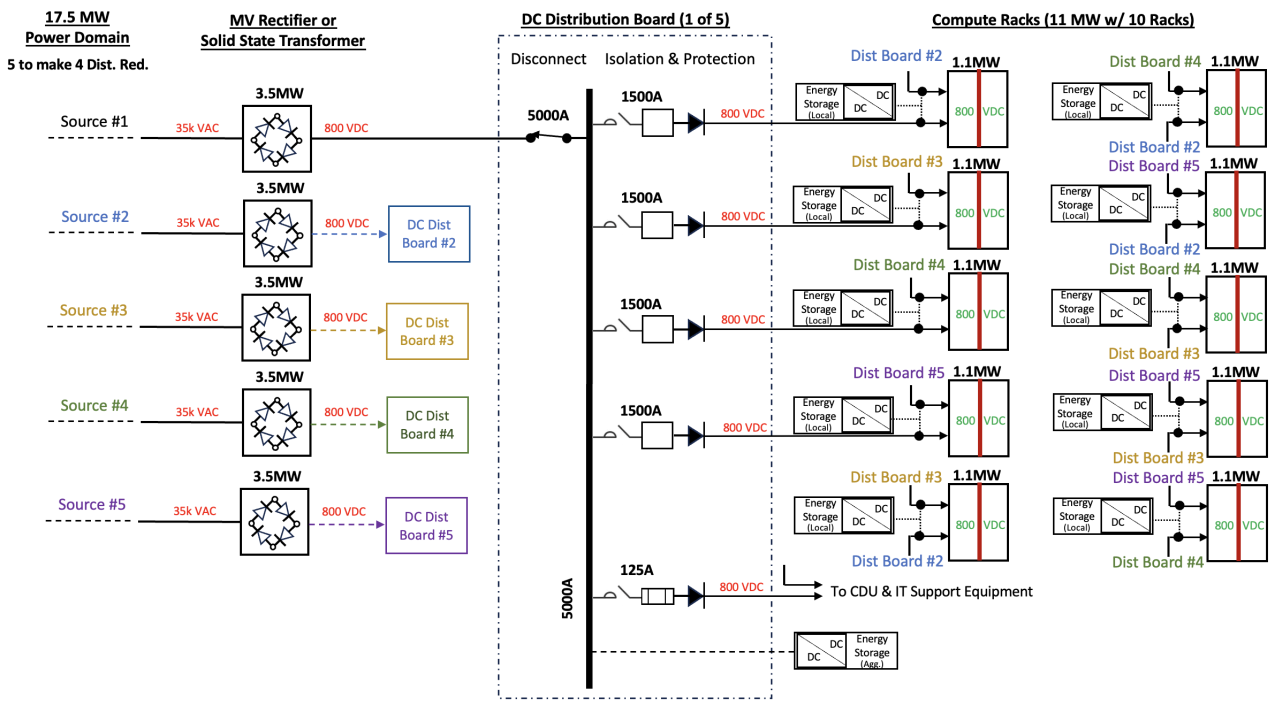
\includegraphics[width=0.8\textwidth]{figures/figure_p16_i1.png}
\caption{800 VDC 17.5 MW Power Block Illustration}
\label{fig:power-block}
\end{figure}

As shown in Figure~\ref{fig:power-block}, the proposed conceptual electrical architecture supports scalable and resilient AI Factory deployment through a 17.5 MW power block leveraging five 3.5 MW medium-voltage (MV) rectifiers in a ``5-to-make-4'' redundant configuration. Each rectifier converts 35 kVAC to 800 VDC and feeds a centralized 5000 A DC distribution board.

Power is distributed via 1500 A busducts or liquid-cooled cables, each equipped with a load-break contactor, solid-state circuit breaker, and blocking diode to ensure safe isolation, fault protection, and containment of fault currents. The system delivers power to four 1.1 MW compute racks along with associated CDUs and IT support equipment.

Each compute rack is supported by local or aggregated energy storage to provide slew-rate control, power smoothing, voltage regulation, and optional backup capability. To maintain concurrent serviceability and uptime, racks are configured with 1+1 redundant feeds sourced from independent rectifiers.

In the event of a single rectifier failure (e.g., loss of Source \#2), the system automatically transfers load to an alternate source, ensuring uninterrupted operation. Even under worst-case loading, a single rectifier (e.g., Source \#1) can sustain up to 3.3 MW of compute load. This demonstrates full-load survivability and readiness for high-density, mission-critical AI workloads.

\section*{Key Design Principles}

\begin{enumerate}
\item \textbf{Modularity:} 3.5 MW rectifier blocks can be paralleled to achieve arbitrary total capacity while maintaining N+1 or N+X redundancy.

\item \textbf{Resilience:} Dual-feed architecture with automatic transfer ensures continuous operation during single-component failures.

\item \textbf{Scalability:} Busduct or liquid-cooled cable distribution supports easy expansion by adding rectifier strings and compute racks.

\item \textbf{Energy Storage Integration:} Built-in support for both short-duration (capacitor) and long-duration (BESS) storage at rack and facility levels.

\item \textbf{Grid Compatibility:} Integrated load-break contactors, solid-state breakers, and blocking diodes ensure compliance with utility interconnection requirements.
\end{enumerate}

\section*{Operational Considerations}

\begin{itemize}
\item \textbf{Maintenance:} Hot-swappable rectifier modules and isolated DC distribution boards enable component-level maintenance without rack downtime.

\item \textbf{Monitoring:} Distributed sensors and smart breakers provide real-time visibility into power flow, fault conditions, and system health.

\item \textbf{Safety:} Touch-safe connectors, mechanical interlocks, and reinforced isolation protect maintenance personnel during servicing.

\item \textbf{Thermal Management:} Liquid-cooled distribution components and rack-level CDUs manage the high heat flux from megawatt-scale compute loads.
\end{itemize}

\section{Industry Collaboration and Path Forward}

To realize this architecture requires multiple points of collaboration with the industry moving forward.

\subsection*{Align on Common Voltage Ranges, Connectors, and Current Levels}

Establishing standardized voltage levels, current ratings, and connector interfaces is essential to enabling modular and interoperable solutions across vendors and system integrators. For AI Factories adopting 800 VDC architectures, industry-wide alignment will minimize customization, accelerate time-to-deploy, and support scalability. A consistent framework allows for flexible deployment strategies while reducing complexity in design, installation, and maintenance.

\subsection*{Develop and Certify DC-Native Equipment}

The transition to facility-level DC distribution requires a new generation of DC-native equipment including rectifiers, distribution systems, protective devices, cabling, connectors, transfer trip schemes and metering. Coordinated development and certification efforts are needed to meet performance, safety, and reliability expectations for data center environments. Collaboration with equipment manufacturers and testing agencies is critical to expedite validation processes and build confidence in large-scale DC power adoption.

Key equipment categories requiring standardization:
\begin{itemize}
\item Medium-voltage to 800 VDC rectifiers (3.5--7.5 MVA range)
\item DC distribution boards with solid-state breakers
\item DC-optimized busducts and liquid-cooled cables
\item Touch-safe, mechanically-interlocked connectors for rack interfaces
\item DC-rated switchgear and protection devices
\item Integrated energy storage systems with fast-response controls
\end{itemize}

\subsection*{Align Safety Standards and Operational Practices}

Operating at 800 VDC voltages introduces new safety considerations that must be addressed through industry-aligned standards and procedures. Clear operational guidelines, including maintenance practices, arc flash mitigation, grounding strategies, and training, will ensure safe handling of 800 VDC infrastructure. Industry working groups and regulatory bodies must collaborate to update or expand applicable codes and best practices.

\subsection*{Priority Action Items}

\begin{enumerate}
\item \textbf{Form industry working groups} to define standardized voltage tolerances, connector pinouts, and current ratings for 800 VDC datacenter equipment.

\item \textbf{Accelerate certification programs} for DC-native components through UL, IEC, and other standards bodies.

\item \textbf{Develop reference implementations} for different scale points (1 MW, 10 MW, 100 MW) with documented bills of materials and integration guidelines.

\item \textbf{Establish testing facilities} for validating end-to-end system performance, fault response, and interoperability.

\item \textbf{Create training curricula} for electricians, maintenance staff, and operators on 800 VDC safety and operations.

\item \textbf{Coordinate with utilities} to define interconnection requirements and grid-support capabilities for AI Factory loads.
\end{enumerate}

\section*{Timeline for Adoption}

\begin{description}
\item[Near-term (0--2 years)] Deploy 800 VDC side-power racks and facility rectifiers using existing 1000 V-class components. Focus on pilot deployments and lessons learned.

\item[Mid-term (2--5 years)] Mature DC-native equipment ecosystem, complete certification processes, and establish industry standards. Begin transitioning from side-power to full facility-level 800 VDC distribution.

\item[Long-term (5+ years)] Evaluate migration to 1500 VDC distribution as safety standards solidify and component availability improves. Widespread SST deployment for direct MV-to-800 VDC conversion.
\end{description}

The window for industry alignment is narrow: AI Factory deployments are already underway, and early adopters will define the de facto standards. Proactive collaboration is essential to avoid fragmentation and ensure that the next generation of power infrastructure can keep pace with AI workload demands.

\section{Conclusion}

The exponential increase in GPU power consumption and evolving requirements for power grids and GPU load profiles are driving the need for a new rack and datacenter power architecture. This new architecture will help to reduce system complexity, cost, and improve efficiency.

\subsection*{Key Findings}

\begin{itemize}
\item \textbf{Power Density Explosion:} GPU racks are approaching 100x the power density of traditional web server racks, with generation-over-generation increases of 2x--8x due to NVLink domain scaling.

\item \textbf{Load Swing Challenge:} Synchronized AI workloads create rapid power swings from 30\% to 100\% rack capacity within milliseconds, requiring multi-timescale energy storage to protect both the grid and compute infrastructure.

\item \textbf{800 VDC Optimality:} 800 VDC distribution offers 157\% more power throughput than 415 VAC over the same conductor area, eliminates unnecessary conversion stages, and aligns with mature EV and industrial DC technologies.

\item \textbf{Dual-Layer Storage:} Facility-level BESS manages minute-scale load averaging and grid transitions, while rack-level capacitors handle sub-100ms GPU power spikes, creating a comprehensive mitigation strategy.

\item \textbf{Architecture Evolution:} The path from 415 VAC \textrightarrow{} 800 VDC side-power \textrightarrow{} facility 800 VDC \textrightarrow{} MV rectifier/SST enables near-term deployment while building toward long-term efficiency gains.

\item \textbf{Industry Imperative:} Standardization of voltage levels, connectors, and safety practices is critical to avoid fragmentation and accelerate ecosystem readiness.
\end{itemize}

\subsection*{Next Steps}

\begin{enumerate}
\item Implement pilot 800 VDC deployments with integrated energy storage to validate reference designs in production environments.

\item Establish industry working groups to define standardized interfaces and safety protocols.

\item Accelerate certification of DC-native equipment through UL, IEC, and other standards bodies.

\item Develop co-ordinated control systems that integrate storage, compute pacing, and grid-forming capabilities.

\item Invest in SST R\&D to enable direct MV-to-800 VDC conversion with compact form factors.
\end{enumerate}

The transition to 800 VDC with integrated energy storage is not optional; it is the architectural foundation required to support the next decade of AI infrastructure growth. Organizations that act now to adopt, standardize, and contribute to this ecosystem will position themselves as leaders in the AI Factory era.

\section*{Acknowledgments}

This document is based on the NVIDIA whitepaper \textit{``800 VDC Architecture for Next-Generation AI Infrastructure''} by Jared Huntington and Mike Tu, which provides the foundational analysis and reference designs for the 800 VDC MGX architecture.


\end{document}
